\documentclass[11pt, a4paper, twoside]{article}   	% use "amsart" instead of "article" for AMSLaTeX format

\usepackage{geometry}                		% See geometry.pdf to learn the layout options. There are lots.
\usepackage{pdfpages}
\usepackage{caption}
\usepackage{minted}
\usepackage[german]{babel}			% this end the next are needed for german umlaute
\usepackage[utf8]{inputenc}
\usepackage{color}
\usepackage{graphicx}
\usepackage{titlesec}
\usepackage{fancyhdr}
\usepackage{lastpage}
\usepackage{hyperref}
\usepackage[autostyle=false, style=english]{csquotes}
\usepackage{mathtools}
\usepackage{tabularx}
% http://www.artofproblemsolving.com/wiki/index.php/LaTeX:Symbols#Operators
% =============================================
% Layout & Colors
% =============================================
\geometry{
   a4paper,
   total={210mm,297mm},
   left=20mm,
   right=20mm,
   top=20mm,
   bottom=30mm
 }	

\definecolor{myred}{rgb}{0.8,0,0}
\definecolor{mygreen}{rgb}{0,0.6,0}
\definecolor{mygray}{rgb}{0.5,0.5,0.5}
\definecolor{mymauve}{rgb}{0.58,0,0.82}

\setcounter{secnumdepth}{4}


% the default java directory structure and the main packages
\newcommand{\srcDir}{../src/}
\newcommand{\imageDir}{./images/}
% =============================================
% Code Settings
% =============================================
\newenvironment{code}{\captionsetup{type=listing}}{}
\newmintedfile[mSourceFile]{matlab}{
	linenos=true, 
	frame=single, 
	breaklines=true, 
	tabsize=2,
	numbersep=5pt,
	xleftmargin=10pt,
	baselinestretch=1,
	fontsize=\footnotesize
}
\newmintinline[mInlineSource]{matlab}{}
\newminted[mSource]{matlab}{
	breaklines=true, 
	tabsize=2,
	autogobble=true,
	breakautoindent=false
}
% =============================================
% Page Style, Footers & Headers, Title
% =============================================
\title{Übung 1}
\author{Thomas Herzog}

\lhead{Data Warehouse}
\chead{}
\rhead{
\includegraphics[scale=0.10]{FHO_Logo_Students.jpg}}

\lfoot{S1610454013}
\cfoot{}
\rfoot{ \thepage / \pageref{LastPage} }
\renewcommand{\footrulewidth}{0.4pt}
% =============================================
% D O C U M E N T     C O N T E N T
% =============================================
% =============================================
% 2016.10.13: 1 
% 2016.10.14: 2
% =============================================

\pagestyle{fancy}
\begin{document}
\setlength{\headheight}{15mm}
%\includepdf[pages={1,2}]{Uebungszettel02.pdf}

\section{Introduction}
This document is the report for the data warehouse part of the lecture \emph{DWO}. Before the \emph{SSIS} and \emph{SSAS} project can be used you need to ensure that the database with name \emph{MDE\_DWO\_WS1617} exists on your local SQL Server instance and has proper permissions set for \emph{SSAS} services user. 
\newline
\newline
The source in the \emph{SSIS} project needs to be modified to point to the proper *.mdb file.

% Section gramar and basics 
\section{Integration Services}
\label{sec:integration-services}
This section deals with the \emph{SSIS Integration Services} part of the hands on. The image \ref{fig:is-control-flow} shows the implemented \emph{Control Flow}. The container \emph{Database Preparation Sequence} holds the components for drop create the warehouse tables which was useful during the development.

\begin{figure}[h]
\centering
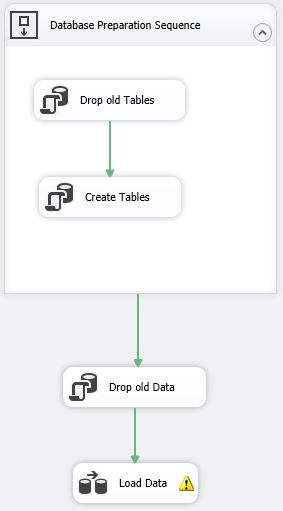
\includegraphics[scale=0.8]{\imageDir/is-control-flow.JPG}
\caption{Integration Service Control Flow}
\label{fig:is-control-flow}
\end{figure}
\ \newline
The following listing describes the components in the control flow:
\begin{itemize}
	\item \emph{Drop old Tables} component drops the existing warehouse tables.
	\item \emph{Create tables} component creates the warehouse tables via an native SQL statement.
	\item \emph{Drop old Data} component drops the old data before data load.
	\item \emph{Load Data} component holds the data flow for data cleanup and restructure.
\end{itemize}
\ \newline
The yellow warn icon is caused by data type changes between the raw data and the prepared data. the data type change is caused by the change of the length of some \emph{nvarchar} typed columns.
\newpage

The image shows the implemented \emph{Data Flow} for the data preparation of the raw data of table \emph{exam} and \emph{student\_group} which will be represented by the tables \emph{exam} and \emph{student} in the warehouse.

\begin{figure}[h]
\centering
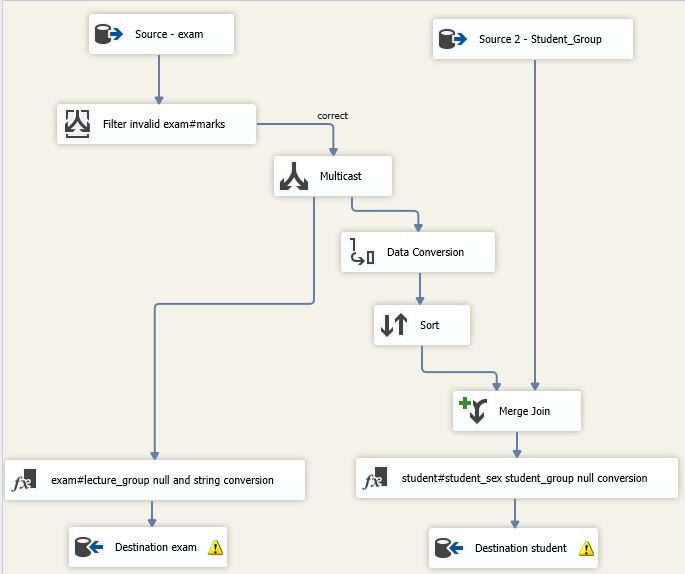
\includegraphics[scale=0.8]{\imageDir/is-data-flow-exam-student.JPG}
\caption{Integration Service Data Flow for \emph{exam}}
\label{fig:is-data-flow-exam}
\end{figure}
\ \newline
The exam input stream gets duplicated for the \emph{student} stream because there are some students in the \emph{exam} table which are not present in the \emph{student\_group} table, therefore the missing students need to be captured from the cleaned up \emph{exam} stream. There are also some students in the \emph{student\_group} table, which have no exam entries, but they are considered to be worthless for the further analysis. The \emph{student\_code} column gets interpreted as a \emph{DT\_WSTR} and in the \emph{student} stream as a \emph{four-byte-signed-integer}. Therefore a cast was necessary to get the proper type for the \emph{Merg Join} component. 
\newline
\newline
The yellow warn icon is caused by some data type changes of some columns. For instance \emph{student\_sex} was changed from \emph{nvarchar(2)} to \emph{nchar(1)}.
\newline
\newline
The result are the two tables \emph{exam} and \emph{student} where the \emph{student} table will only contain students which have \emph{exam} entries. Students not present in the \emph{student\_group} table before, will get the \emph{student\_group} set to \emph{U} which stands for unknown. The exam table was cleaned of the attribute \emph{student\_sex} which is part of the table \emph{student}.
\newpage

The image shows the implemented \emph{Data Flow} for the data preparation of the raw data of table \emph{lehrer\_prod} and \emph{teacher\_group} which will be represented by the tables \emph{teacher} in the warehouse.

\begin{figure}[h]
\centering
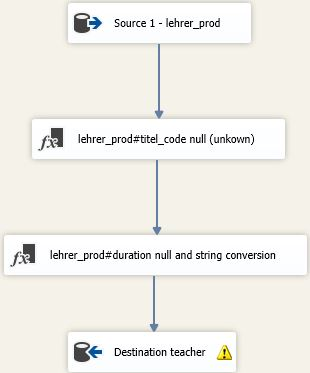
\includegraphics[scale=0.8]{\imageDir/is-data-flow-teacher.JPG}
\caption{Integration Service Data Flow for \emph{lehrer\_prod} and \emph{teacher\_group}}
\label{fig:is-data-flow-teacher}
\end{figure}
\ \newline
The \emph{teacher\_group} and \emph{lehrer\_prod} tables get merged to the \emph{teacher} table. If teachers are missing in the \emph{teacher\_group} table or the \emph{typ} column in the \emph{teacher\_group} table is null, then they get assigned to the group \emph{unknown}. The duration gets converted to a string of the form \emph{Duration 1} or to \emph{unknown} if no duration is present.
\newline
\newline
The yellow warn icon is caused by some data type changes of some columns. For instance \emph{teacher\_sex} was changed from \emph{nvarchar(2)} to \emph{nchar(1)}.
\newline
\newline
The result is the table \emph{teacher} which holds all teachers present in the \emph{exam} table with all their attributes.

\newpage

\section{Analysis Services}
This section deals with the \emph{SSAS Analysis Services} part of the hands on. 

\subsection{Implemented Project}
This section deals with the implemented project for the analysis part of the hands on.

\begin{figure}[h]
\centering
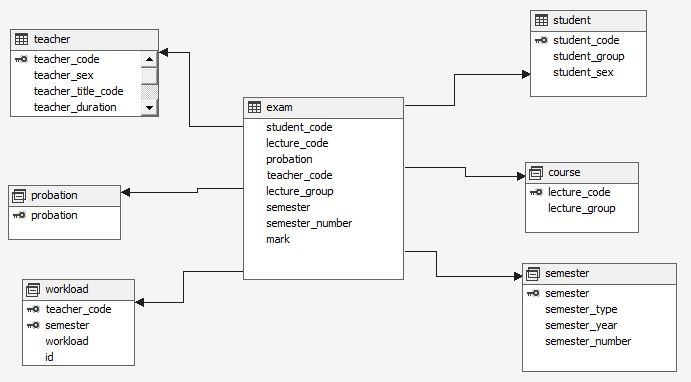
\includegraphics[scale=0.7]{\imageDir/as-data-source-view.JPG}
\caption{Data source view of the warehouse database}
\label{fig:is-data-flow-teacher}
\end{figure}
\ \newline
The tables \emph{workload}, \emph{probation}, \emph{course} and \emph{semester} were create as named queries.

\begin{figure}[h]
\centering
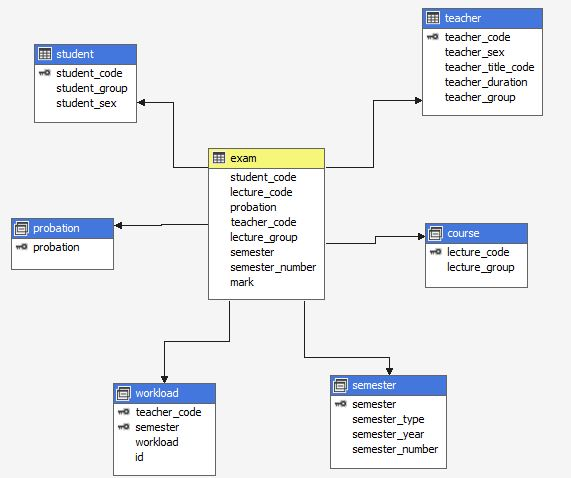
\includegraphics[scale=0.7]{\imageDir/as-cube.JPG}
\caption{Implemented cube}
\label{fig:is-data-flow-teacher}
\end{figure}
\ \newpage

\begin{figure}[h]
\centering
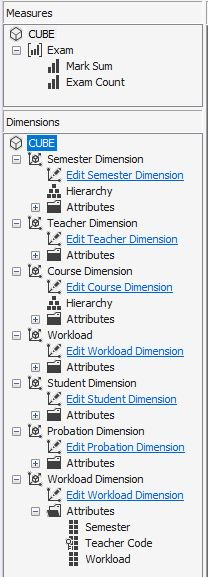
\includegraphics[scale=0.7]{\imageDir/as-measures-dimensions.JPG}
\caption{Cube measures and dimensions}
\label{fig:is-data-flow-teacher}
\end{figure}

\begin{figure}[h]
\centering
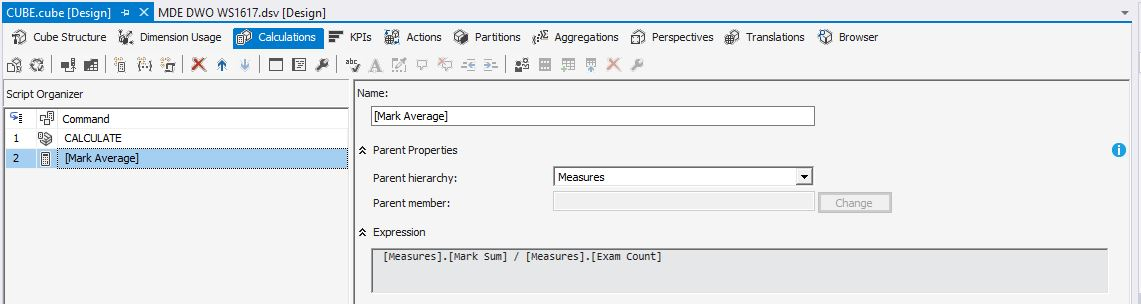
\includegraphics[scale=0.6]{\imageDir/as-calculated-member.JPG}
\caption{Cube measures and dimensions}
\label{fig:is-data-flow-teacher}
\end{figure}
\ \newpage

\subsection{Reports}
The following images are showing the result of the made reports based on the implemented cube.

\begin{figure}[h]
\centering
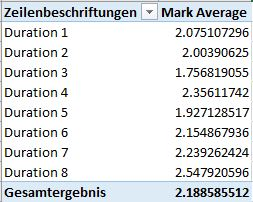
\includegraphics[scale=0.9]{\imageDir/report-teacher-seniority.JPG}
\caption{Report Teachers seniority}
\label{fig:is-data-flow-teacher}
\end{figure}

\begin{figure}[h]
\centering
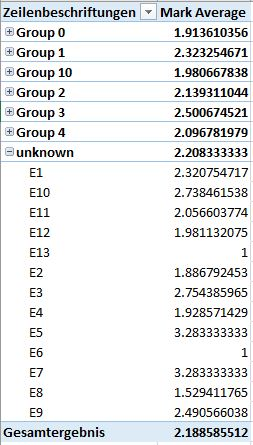
\includegraphics[scale=0.8]{\imageDir/report-course-type.JPG}
\caption{Report Course type}
\label{fig:is-data-flow-teacher}
\end{figure}
\ \newpage

\begin{figure}[h]
\centering
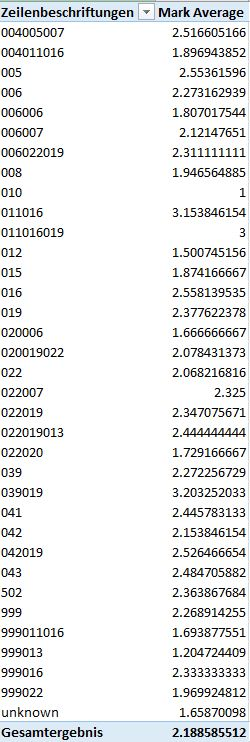
\includegraphics[scale=0.8]{\imageDir/report-teacher-title.JPG}
\caption{Report Teacher job title}
\label{fig:is-data-flow-teacher}
\end{figure}
\ \newpage

\begin{figure}[h]
\centering
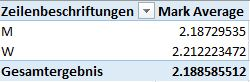
\includegraphics[scale=0.8]{\imageDir/report-teacher-sex.JPG}
\caption{Report Teacher sex}
\label{fig:is-data-flow-teacher}
\end{figure}

\begin{figure}[h]
\centering
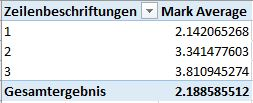
\includegraphics[scale=0.8]{\imageDir/report-probation.JPG}
\caption{Report Probation}
\label{fig:is-data-flow-teacher}
\end{figure}

\begin{figure}[h]
\centering
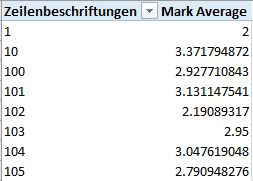
\includegraphics[scale=0.8]{\imageDir/report-teacher-code.JPG}
\caption{Report teacher code (truncated)}
\label{fig:is-data-flow-teacher}
\end{figure}
\ \newpage

\begin{figure}[h]
\centering
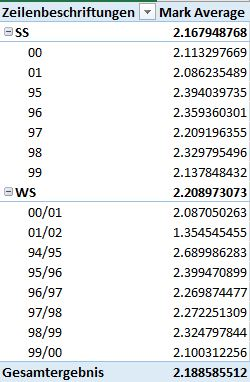
\includegraphics[scale=0.8]{\imageDir/report-over-time.JPG}
\caption{Report over time (semesters)}
\label{fig:is-data-flow-teacher}
\end{figure}

\begin{figure}[h]
\centering
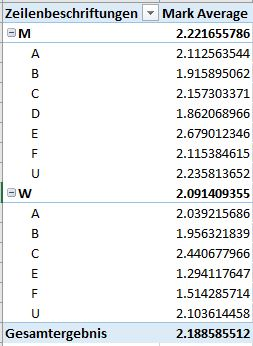
\includegraphics[scale=0.8]{\imageDir/report-student-to-student-group.JPG}
\caption{Report student and student group}
\label{fig:is-data-flow-teacher}
\end{figure}
\ \newpage

\begin{figure}[h]
\centering
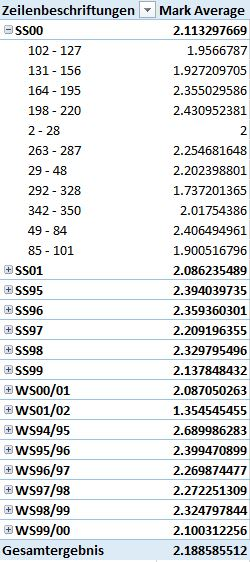
\includegraphics[scale=0.8]{\imageDir/report-workload.JPG}
\caption{Report workload over semesters}
\label{fig:is-data-flow-teacher}
\end{figure}

\begin{figure}[h]
\centering
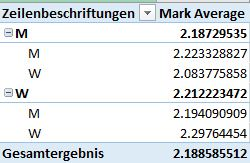
\includegraphics[scale=0.8]{\imageDir/report-teacher-to-student-sex.JPG}
\caption{Report teacher and student sex}
\label{fig:is-data-flow-teacher}
\end{figure}
\ \newpage

\end{document}
